\newthought{\textbf{Rizki Ilhami - 2020903430042 - TRKJ 3B}}

\newday{\textbf{1 - 2 Desember 2022} - Instalasi dan Konfigurasi Hadoop}

\begin{enumerate}

\item Kendala dan Solusi
\begin{enumerate}
    \item kendala
\begin{itemize}
    \item Kendalanya pada saat menjalankan hadoop service, firefox tidak bisa dibuka.
\end{itemize}
    \item solusi
\begin{itemize}
    \item menginstal ulang firefox.
\end{itemize}
\end{enumerate}

\item Kesimpulan
\newline
    Pada Instalasi Apache Hadoop membutuhkan ruang yang
    cukup besar untuk mengekstrak file Apache Hadoop dan ram
    minimal 2gb agar bekerja optimal.


\begin{figure}[!ht]
    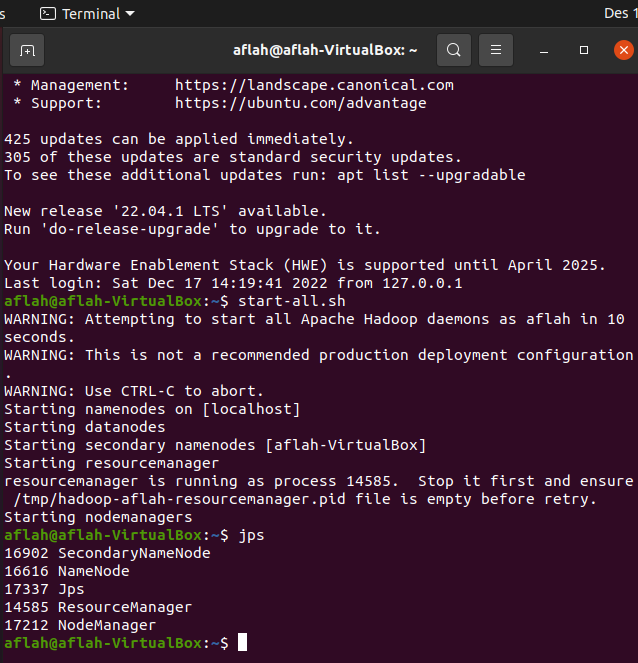
\includegraphics[width=\textwidth]{RizkiIlhami/jps}
    \caption{hasil jps}
    \label{gam:Hasil}
\end{figure}

\begin{figure}[!ht]
    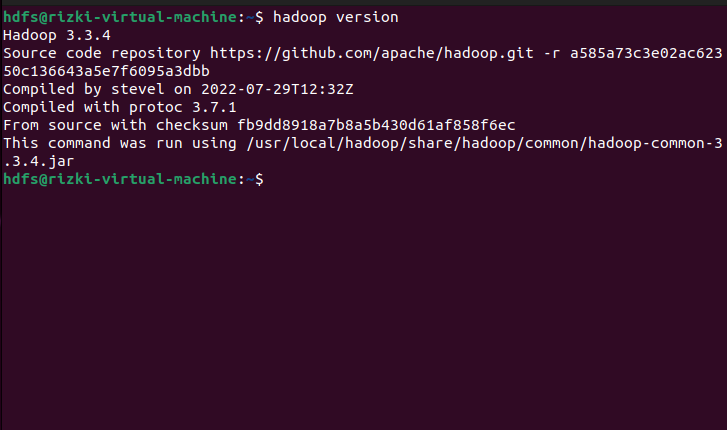
\includegraphics[width=\textwidth]{RizkiIlhami/Hadoop Version}
    \caption{hasil Hadoop}
    \label{gam:Hasil}
\end{figure}

\begin{figure}[!ht]
    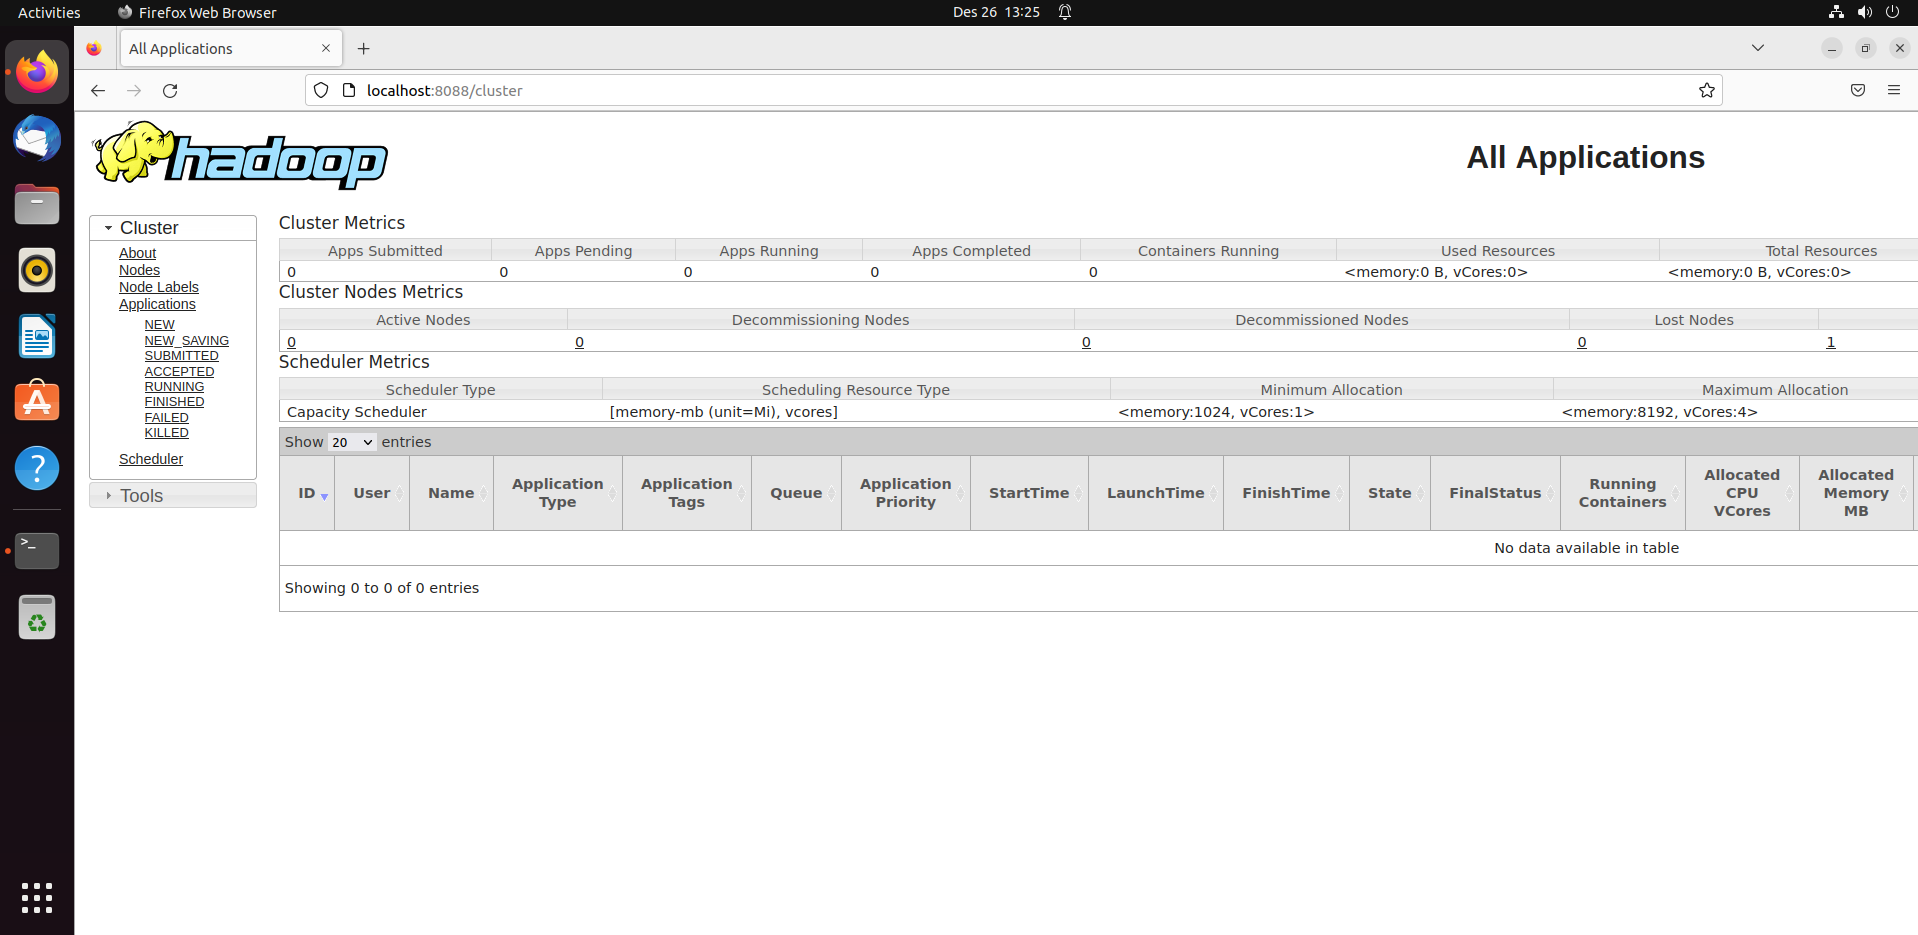
\includegraphics[width=\textwidth]{RizkiIlhami/Hadoop Web}
    \caption{hasil menjalankan Hadoop Service}
    \label{gam:Hasil}
\end{figure}

\end{enumerate}

\clearpage
\newday{\textbf{8 Desember 2022} - WordCount bawaan Hadoop}
\begin{enumerate}
\item Kendala dan Solusi

\begin{itemize}
\item Tidak menemukan kendala apapun.
\end{itemize}

\item Kesimpulan
\newline
    Pada Hadoop terdapat program untuk menghitung jumlah kata 
    (WordCount) yang ada pada data. Sebagai praktikan melakukan input data terlebih
    dahulu, kemudian memprosesnya, sehingga menghasilkan data output.

\end{enumerate}

\begin{figure}[!ht]
    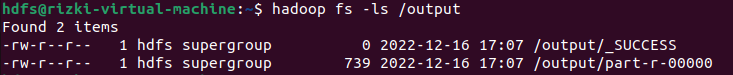
\includegraphics[width=\textwidth]{RizkiIlhami/WordCount Hadoop -ls}
    \caption{hasil WordCount bawaan hadoop}
    \label{gam:Hasil}
\end{figure}

\begin{figure}[!ht]
    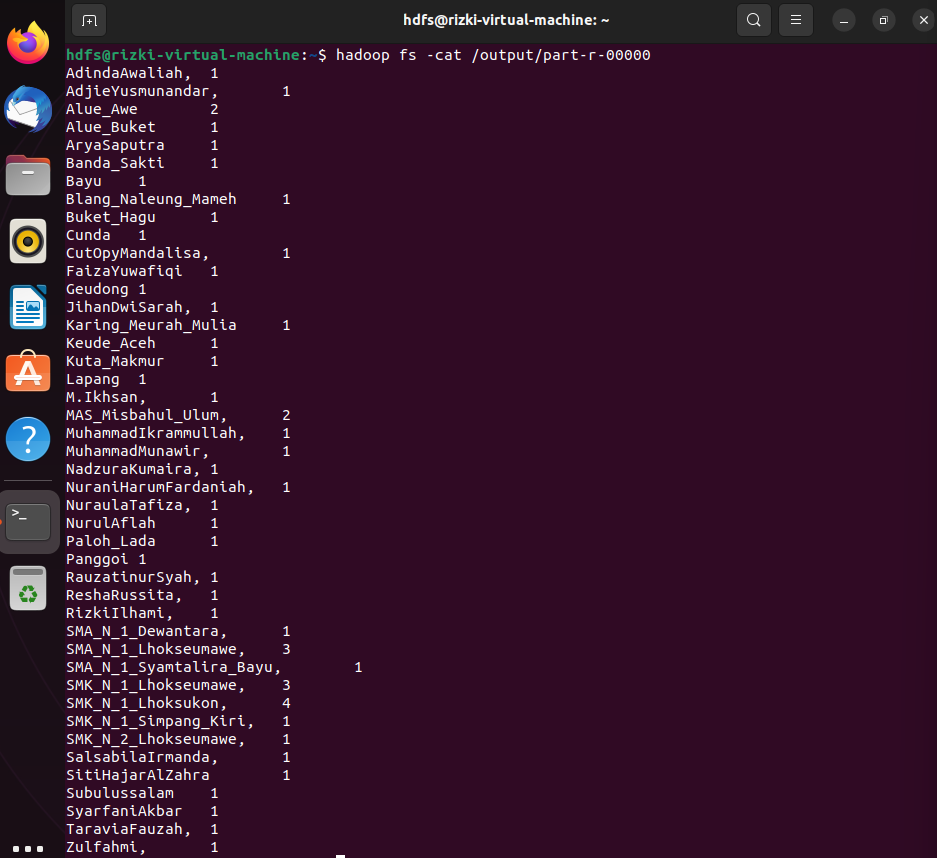
\includegraphics[width=\textwidth]{RizkiIlhami/WordCount Hadoop -cat}
    \caption{hasil WordCount bawaan hadoop}
    \label{gam:Hasil}
\end{figure}

\clearpage
\newday{\textbf{9 Desember 2022} - WordCount dengan Java}
\begin{enumerate}
\item Kendala dan Solusi

\begin{itemize}
\item Tidak menemukan kendala apapun.
\end{itemize}

\item Kesimpulan
\newline
    Untuk hasil yang ditampikan sama dengan WordCount bawaan hadoop.

\end{enumerate}

\begin{figure}[!ht]
    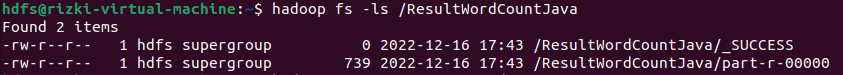
\includegraphics[width=\textwidth]{RizkiIlhami/WordCount Java -ls}
    \caption{hasil WordCount Java}
    \label{gam:Hasil}
\end{figure}

\begin{figure}[!ht]
    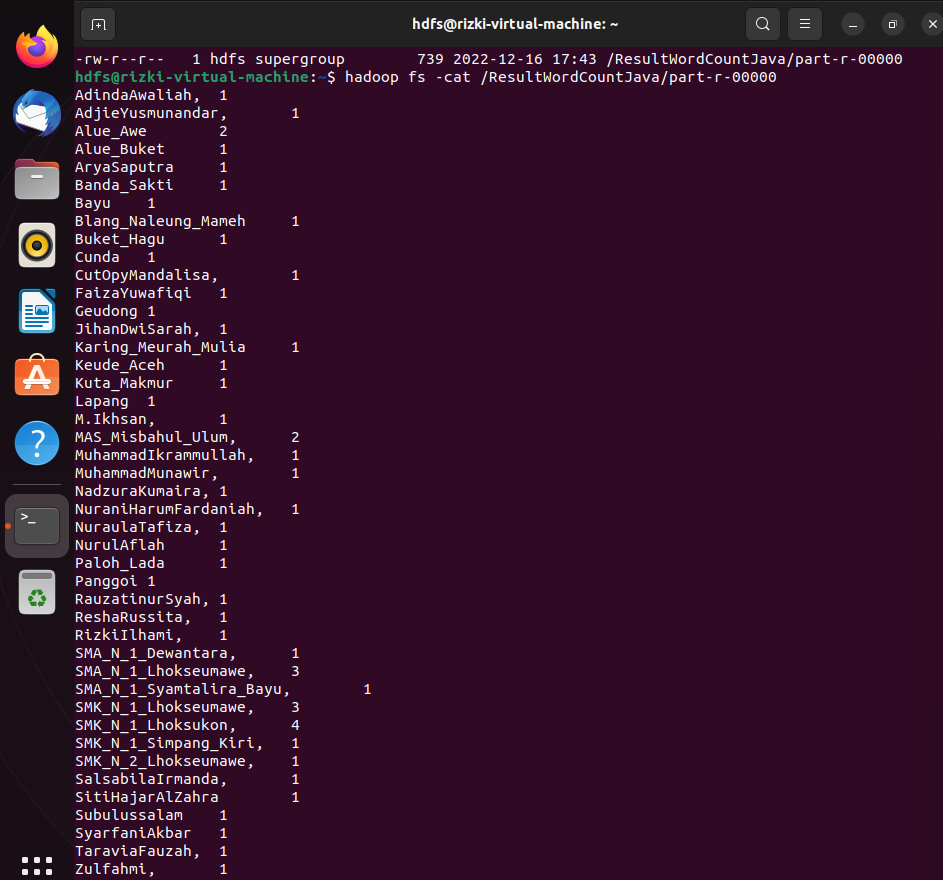
\includegraphics[width=\textwidth]{RizkiIlhami/WordCount Java -cat}
    \caption{hasil WordCount Java}
    \label{gam:Hasil}
\end{figure}


\clearpage
\newday{\textbf{15 Desember 2022} - Instalasi Apache Spark}
\begin{enumerate}
\item Kendala dan Solusi

\begin{itemize}
\item Tidak menemukan masalah apapun
\end{itemize}


\item Kesimpulan
\newline
    Apache Spark adalah sebuah framework komputasi
    yang dapat digunakan untuk mengakses data, memproses
    data, menanyakan data serta menganalisis big data

\end{enumerate}

\begin{figure}[!ht]
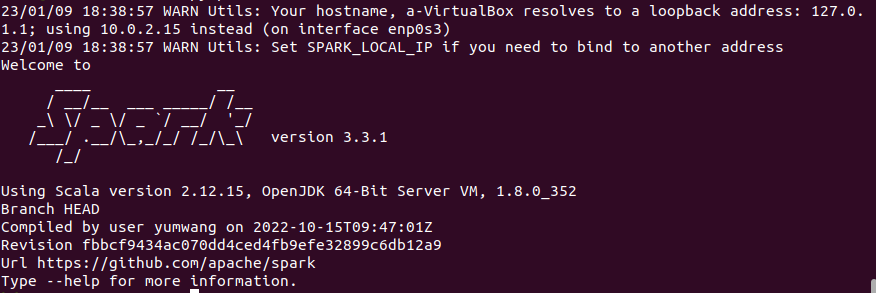
\includegraphics[width=\textwidth]{RizkiIlhami/spark}
\caption{hasil instalasi apache spark }
\label{gam:hasil instalasi spark}
\end{figure}

\clearpage
\newday{\textbf{16 Desember 2022} - WordCount Dengan Python}
\begin{enumerate}
\item Kendala dan Solusi

\begin{enumerate}
    \item kendala
\begin{itemize}
    \item Tidak bisa menjalankan {\color{red}"echo jangan heran jika orang cantik merasa jelek sementara
    orang yang jelek merasa cantik | WordCountPython/map.py |
    sort | WordCountPython/reduce.py"}
\end{itemize}
    \item solusi
\begin{itemize}
    \item Memeriksa pada {\color{red}file map.py} dan {\color{red}reduce.py}
    \item Setelah diteliti lebih mendalam ternyata ada tulisan yang keliru dan ada yang perlu ditambah lagi.
\end{itemize}
\end{enumerate}

\item Kesimpulan
\newline Berhasil menjalankan program WordCountPython dengan baik, walaupun banyak kendala yang dialami.


\begin{figure}[!ht]
    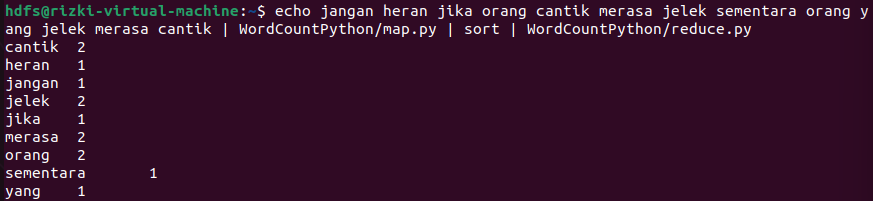
\includegraphics[width=\textwidth]{RizkiIlhami/WordCount python step 6}
    \caption{Mencoba program di local }
    \label{gam:hasil WordCountPython}
    \end{figure}

\begin{figure}[!ht]
    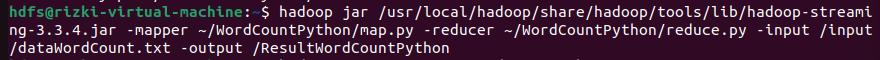
\includegraphics[width=\textwidth]{RizkiIlhami/WordCount python step 7}
    \caption{Menjalankan Program menggunakan Hadoop }
    \label{gam:hasil WordCountPython}
\end{figure}

\begin{figure}[!ht]
    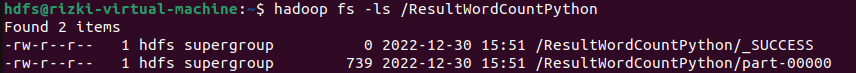
\includegraphics[width=\textwidth]{RizkiIlhami/WordCount python step 8}
    \caption{Hasil WordCount Python }
    \label{gam:hasil WordCountPython}
\end{figure}

\begin{figure}[!ht]
    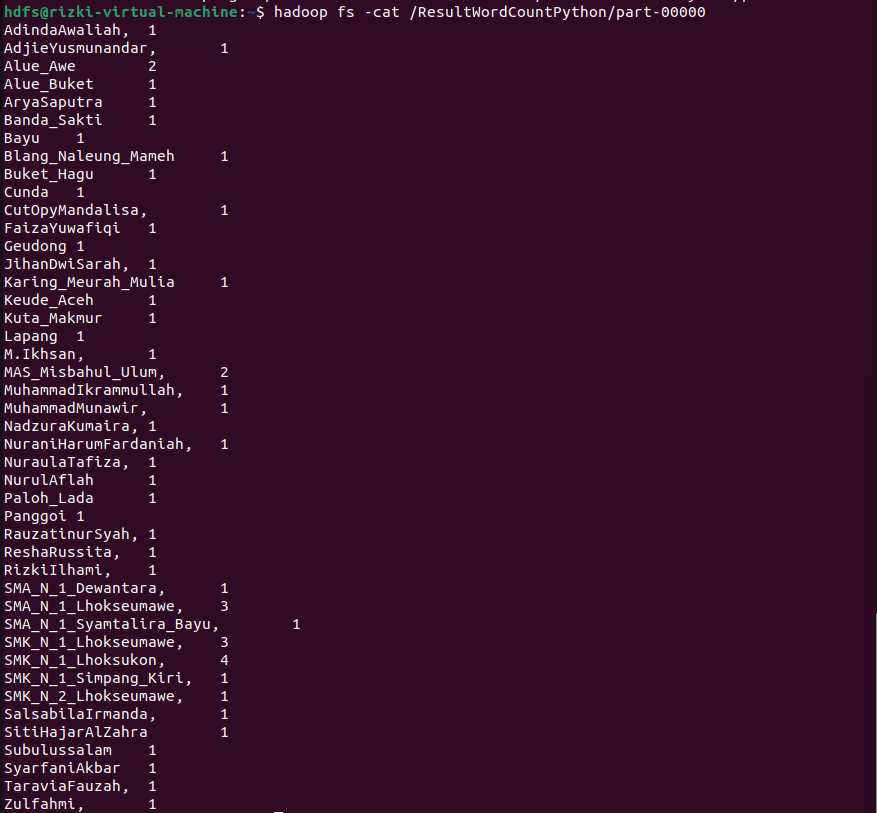
\includegraphics[width=\textwidth]{RizkiIlhami/WordCount python step 9}
    \caption{Hasil WordCount Python }
    \label{gam:hasil WordCountPython}
\end{figure}

\end{enumerate}

\clearpage
\newday{\textbf{22 Desember 2022} - WordCount dengan PySpark}
\begin{enumerate}
\item Kendala dan Solusi

\begin{enumerate}
    \item kendala
\begin{itemize}
    \item Tidak bisa menjalankan perintah 
    {\color{red}"hadoop fs -ls /ResultWordCountPyspark"} dan 
    {\color{red}"hadoop fs -cat /ResultWordCountPyspark/part-00000"}
\end{itemize}
    \item solusi
\begin{itemize}
    \item Mengecek ulang file {\color{red}WordCount.Py} dan menemukan kekeliruan pada tanda petik (').
    \item Terdapat kesalahan pada saat membuat perintah pada huruf bersar dan kecil.
\end{itemize}
\end{enumerate}

\item Kesimpulan
\newline Program Berhasil berjalan walau ada sedikit kendala yang saya alami.

\end{enumerate}

\begin{figure}[!ht]
    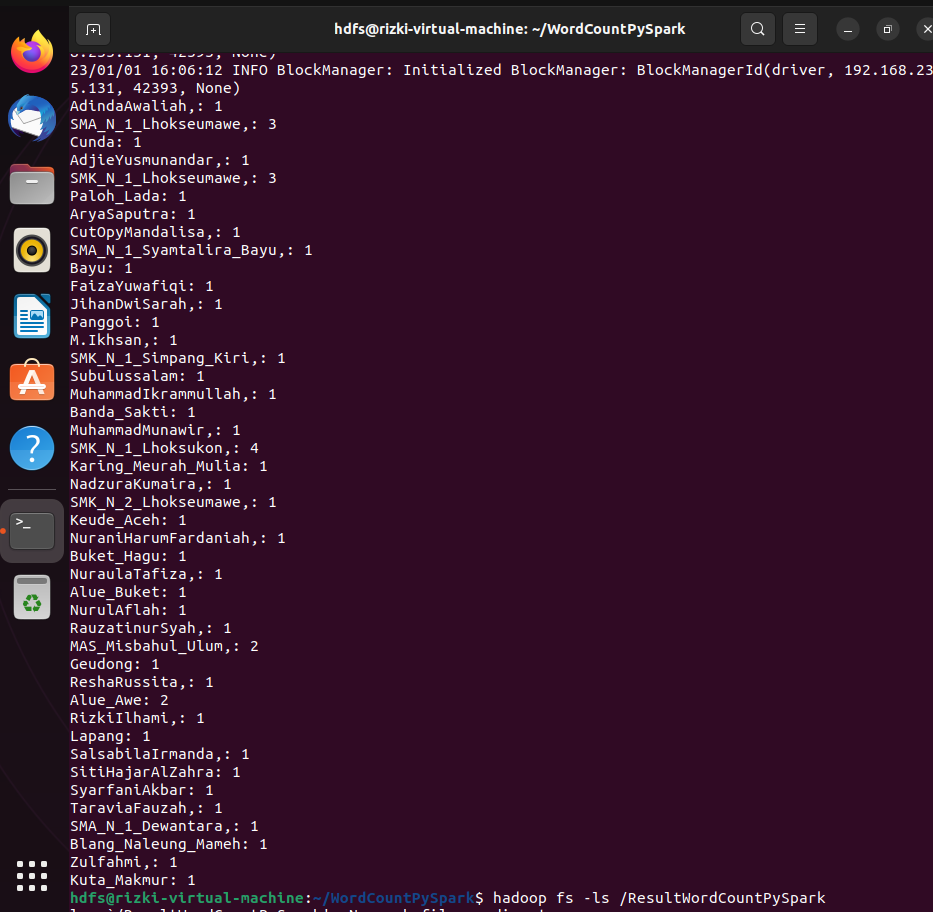
\includegraphics[width=\textwidth]{RizkiIlhami/Pyspark}
    \caption{Hasil WordCount PySpark }
    \label{gam:hasil WordCountPyspark}
\end{figure}

\clearpage
\newday{\textbf{23 Desember 2022} - Machine Learning dengan PySpark}
\begin{enumerate}
\item Kendala dan Solusi

\begin{enumerate}
    \item kendala
\begin{itemize}
    \item Bingung dengan cara penulisan kode.
\end{itemize}
    \item solusi
\begin{itemize}
    \item Mencoba dengan banyak percobaan.
\end{itemize}
\end{enumerate}

\item Kesimpulan
\newline Melakukan percobaan dan mengikuti langkah-langkah hingga selesai.
percobaan Berhasil dilakukan walau banyaknya error pada pengetikan kode yang dialami.


\begin{figure}[!ht]
    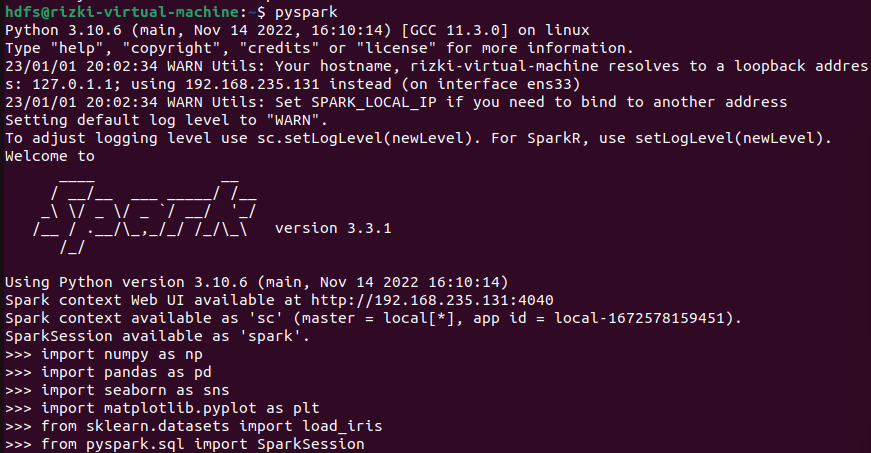
\includegraphics[width=\textwidth]{RizkiIlhami/Learning - Load Package}
    \caption{Load Package}
    \label{gam:hasil Learning}
\end{figure}
	
\begin{figure}[!ht]
    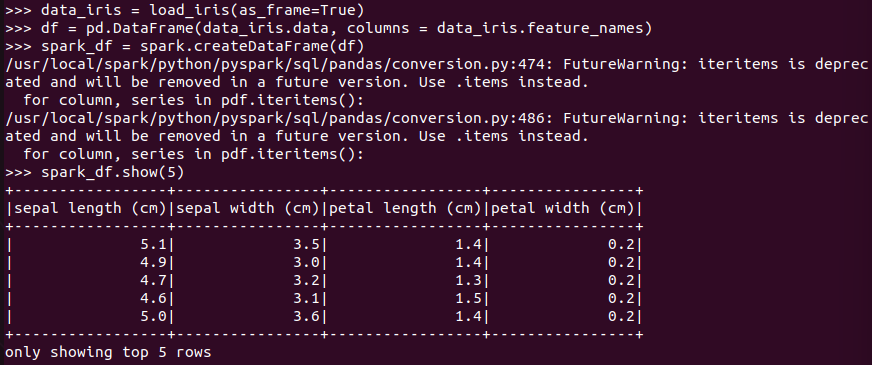
\includegraphics[width=\textwidth]{RizkiIlhami/Learning - Load Data}
    \caption{Load Data}
    \label{gam:hasil Learning}
\end{figure}

\begin{figure}[!ht]
    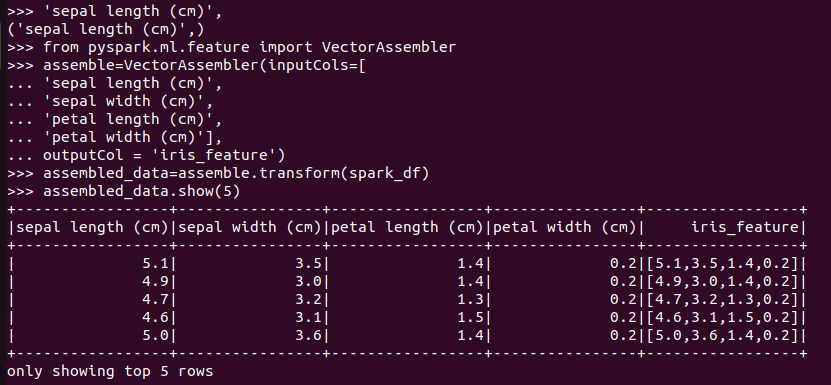
\includegraphics[width=\textwidth]{RizkiIlhami/Learning - metode silhouette}
    \caption{Metode Silhouette}
    \label{gam:hasil Learning}
\end{figure}

\begin{figure}[!ht]
    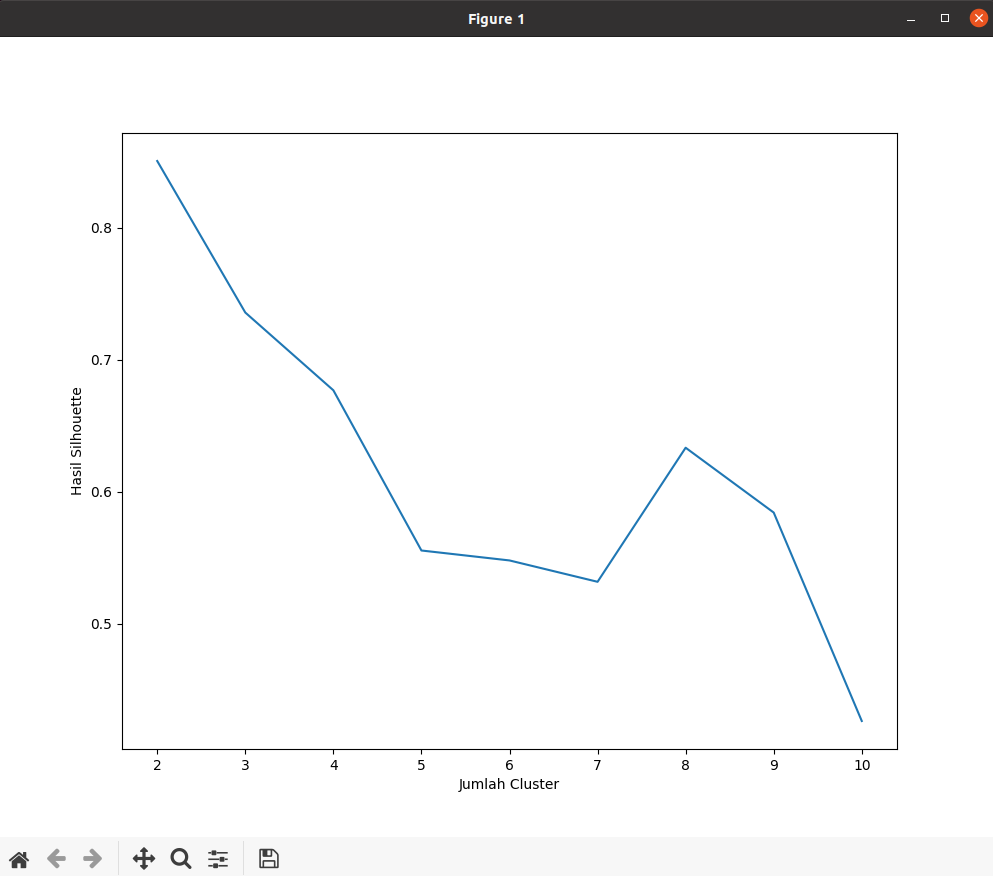
\includegraphics[width=\textwidth]{RizkiIlhami/Learning - silhouette Grafik}
    \caption{Grafik Silhouette}
    \label{gam:hasil Learning}
\end{figure}

\begin{figure}[!ht]
    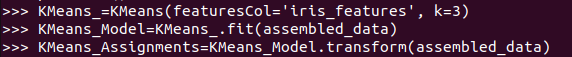
\includegraphics[width=\textwidth]{RizkiIlhami/Learning - K-Means Clustering}
    \caption{Model K-Means Clustering}
    \label{gam:hasil Learning}
\end{figure}

\begin{figure}[!ht]
    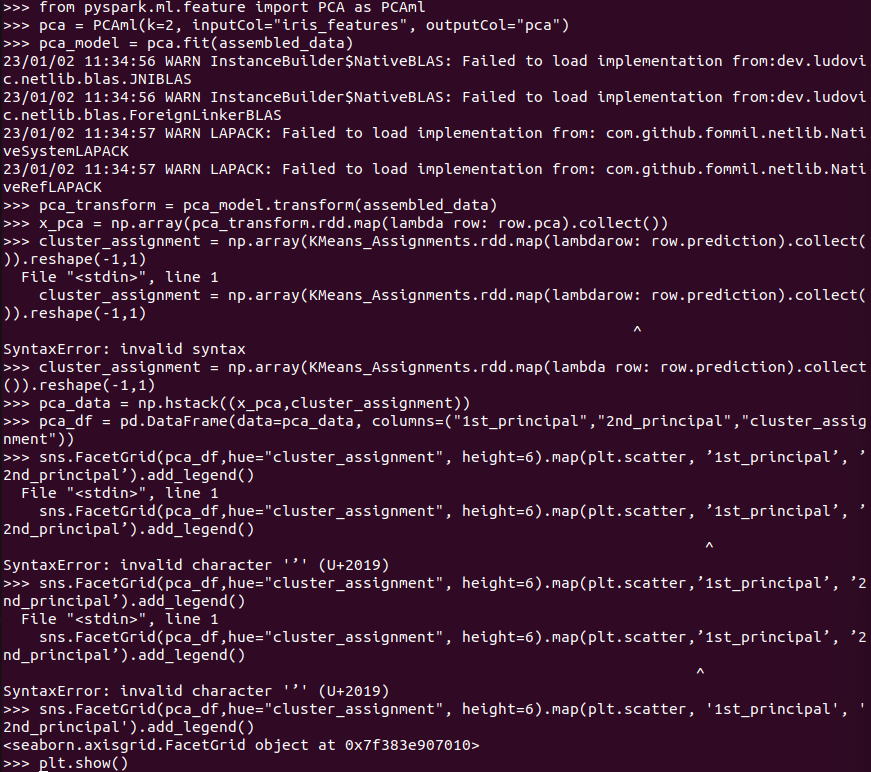
\includegraphics[width=\textwidth]{RizkiIlhami/Learning - Clustering dengan PCA}
    \caption{Clustering dengan PCA}
    \label{gam:hasil Learning}
\end{figure}

\begin{figure}[!ht]
    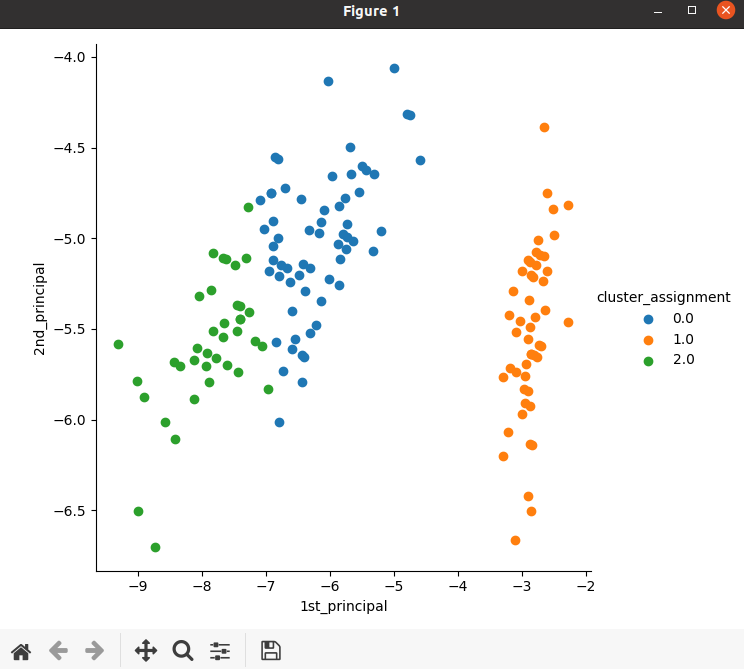
\includegraphics[width=\textwidth]{RizkiIlhami/Learning - Clustering Grafik}
    \caption{Garfik Clustering}
    \label{gam:hasil Learning}
\end{figure}

\end{enumerate}